\subsection{Test af omregning til grader}

For at teste, at omregningen fra spændingen fra accelerometeret til grader fungerer i praksis, bevæges vinkeltesteren, der er vist på \autoref{fig:vinkeltest}, fra $180^{\circ}$ til $70^{\circ}$. Figur \ref{fig:spaending_vinkel_test} illustrer dette i MATLAB, hvor vinklen er illustreret på den venstre y-akse, og hvor accelerometrenes spænding er illustrerede på den højre y-akse. 

\begin{figure}[H]
\centering
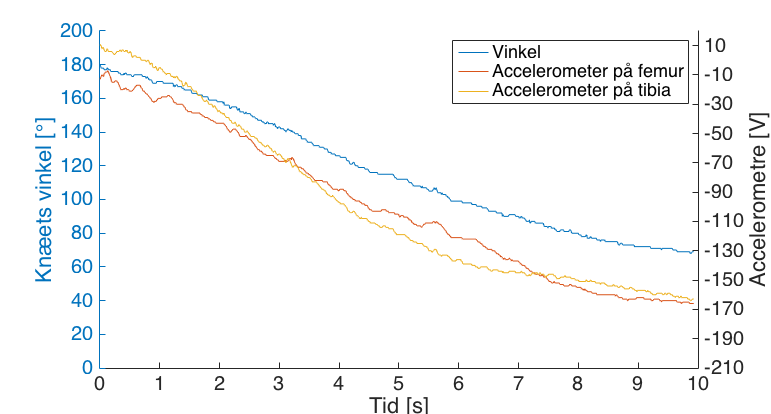
\includegraphics[width=0.8\textwidth]{figures/spaending_vinkel_test}
\caption{Test af grader, hvor vinkeltesteren er instillet til $90^{\circ}$ }
\label{fig:spaending_vinkel_test}
\end{figure}

\noindent
Det ses på \autoref{fig:spaending_vinkel_test}, at omregningen fra spænding til grader forløber som forventet. Der tages udgangspunkt i \autoref{tab:vinkelinterval_psoc} for omregningen, hvor spændingen for hvert accelerometer omregnes til grader, og disse lægges så sammen for at få den samlede vinkel. 

På figuren aflæses, at systemet registrerer en vinkel på $90^{\circ}$, når  accelerometeret på femur giver en spænding på $-136~V$ og accelerometeret på tibia giver en spænding på $-145~V$. Disse spændinger kan omregnes til vinkler ved først at finde, hvad spændingen er for én grad ud fra \autoref{tab:vinkelinterval_psoc}  i dét spændingsinterval, hvori den aflæste spænding befinder sig. Det kan aflæses i tabellen, at spændingen fra accelerometeret på femur giver en vinkel mellem 30 og $50^{\circ}$.

\begin{equation}
\dfrac{-143~V-(-84~V)}{20^{\circ}}=-2,95~V
\end{equation}
Derefter findes vinklen for accelerometeret.

\begin{equation}
\dfrac{-84~V+136~V}{2,95~V}+30^{\circ}=47,627^{\circ}
\end{equation}
Ligeledes kan vinklen fra accelerometeret på tibia udregnes til $41,429^{\circ}$. Dette giver en samlet vinkel over leddet: 
%
\begin{equation}
47,627^{\circ}+41,429^{\circ}=89,056^{\circ}
\end{equation}
Dette giver en afvigelse på $-1,049~\%$ fra de $90^{\circ}$	. Denne afvigelse kan godtages til dette systems formål, da der ikke er nogen fare forbundet med, at systemet overskrider de opstillede grænser for vinkler med $-1,049~\%$.









